\documentclass[12pt]{article}
\usepackage{color}
\usepackage[usenames,dvipsnames,svgnames,table]{xcolor}
\definecolor{dark-red}{rgb}{0.7,0.1,0.1} 
\definecolor{dark-blue}{rgb}{0,0,0.7} 
\usepackage[linkcolor=dark-red,
            colorlinks=true,
            urlcolor=dark-blue,
            pdfstartview={XYZ null null 1.00},
            pdfauthor={Gaurav Sood and Andy Guess, gsood07@gmail.com},
            citecolor=dark-red,
            bookmarks=false,
            pdfborder={0 0 0},
            pdftitle={Precise Numerical Summaries}]{hyperref}
            
\usepackage{amsfonts,amssymb,amsbsy,amsmath,amsxtra}

\usepackage[letterspace=500]{microtype}
\usepackage{libertine}
\usepackage[T1]{fontenc}

\usepackage{indentfirst}
\usepackage{setspace} % To set line spacing
\usepackage{multirow}

\usepackage{verbatim}

\usepackage[multiple]{footmisc}
\usepackage{fancyvrb}

\usepackage{longtable}

\usepackage[margin=1in]{geometry}
\usepackage{graphicx}

\raggedright
\parindent=1.5em % <- or whatever indent you want

\usepackage{natbib}
\usepackage{url}
\begin{comment}

setwd(paste0(basedir, "quant-discipline/ms"))
tools::texi2dvi("quant.tex", pdf=TRUE, clean=TRUE) 
setwd(basedir)

\end{comment}

\begin{document}
\title{\vspace{-.5cm}\large{\textbf{By the Numbers: Toward More Precise Numerical Summaries}}\footnote{We thank Justin Esarey, Andrew Gelman, Don Green, Kabir Khanna, Brendan Nyhan, and Daniel Stone for useful comments. The data and the scripts behind the analysis presented here can be downloaded at: \url{http://github.com/soodoku/quant-discipline/}}\vspace{.5cm}}
\author{Gaurav Sood\footnote{Gaurav is a data scientist. He can be reached at: \href{mailto:gsood07@gmail.com}{\small{gsood07@gmail.com}}} \and Andrew Guess\footnote{Andrew is a Postdoctoral Fellow  at the Social Media and Political Participation (SMaPP) Lab, New York University. He can be reached at: \href{mailto:guess@nyu.edu}{\small{guess@nyu.edu}}}}
\date{\vspace{.5cm}\normalsize{\today}} 
\maketitle
\doublespacing

Unlike the natural sciences, there are few true zeros in the social sciences \citep[p. 960,][]{gelman2011causality}. All sorts of variables are often weakly related to each other. And however lightly social scientists, exogenous events, or other actors intervene, effects of those interventions are rarely precisely zero. When there are few true zeros, categorical statements, like ``two variables are significantly related'' or ``the intervention had a significant effect,'' convey limited information---about sample size and luck (and manufactured luck). Yet these kinds of statements are the norm in abstracts of the top political science journal, the \emph{American Political Science Review} (\emph{APSR}).  As we show later, only 10\% of the empirical articles in recent volumes of \emph{APSR} have abstracts with precise quantitative statements. The comparable number for the \emph{American Economic Review} (\emph{AER}) is 35\%.

Informal inspection also suggests that coarse descriptions are common in other sections of social science articles, aside from being exceedingly frequent in the social science vernacular. (We would like to quantify both.) Studies are often summarized as ``the study shows this broad phenomenon exists.'' For instance, \citet{pasek2015} write, ``Moreover, much past research shows that guessing is often biased.'' Surprisingly, and more problematically, comparison of results often enough also takes the same form. For instance, a study on motivated learning contextualizes the results as follows: ``Our finding is consistent with other research showing that even when people agree on factual information, they often still interpret the information in a motivated manner'' (from \citealt{khanna2015}). The phrase ``finding is consistent with'' yields nearly 300,000 results on Google Scholar. And informal inspection suggests that ``consistent'' covers a surprisingly large range of effect sizes and measures.    

None of this is to say that the decision to imprecisely summarize is made without deliberation. Undoubtedly, some resort to coarse summaries because they are not confident about their theories, measures, or models. Others likely use coarse summaries because they think coarse summaries are a more effective way to communicate. In fact, there is some support for the basis for such a thesis. A survey of undergraduate and graduate students found that 77\% of the students thought that people preferred to receive verbal expressions of uncertainty over numerical expressions in their everyday lives \citep{wallsten1993preferences}. (However, the paper also notes that 85\% of the students felt comfortable switching to another mode if they thought the other mode suited their needs better.)  

Our hunch, however, is that the most common form of coarse summaries in scientific communication---categorical statements around statistical significance---arise as a natural consequence of scientists thinking in terms of the Null Hypothesis Statistical Testing (NHST) framework, which in turn is likely underpinned by a Popperian understanding of science \citep{gelman2013philosophy}. For instance, hypotheses in the form of coarse categorical statements like, ``X will be positively associated with Y,'' are exceedingly frequent. These kinds of hypotheses reflect an understanding of science in which  scientific progress comes from falsification rather than from improvements in measurement. 

Whatever the root cause, the use of coarse summaries likely leads to serious problems. First, coarse summarizations risk misinterpretation. Partly because the mapping between verbal phrases and numerical ranges varies between communicators and recipients \citep{capriotti2011miscommunication}, numbers that verbal expressions are mapped to vary a great deal \citep{beyth1982probable, bocklisch2010role, brun1988verbal, simpson1944specific, simpson1963stability}. For instance, \citet{beyth1982probable} elicited numerical mappings of 30 verbal expressions on a 100-point scale and found that the average inter-quartile range of the numerical mapping for a phrase was 14.4. Analogous numbers---standard deviations of the numerical mappings---from \citet{brun1988verbal}, based on 27 phrases, and \citet{bocklisch2010role}, based on 13 phrases, were 14.2\% (translated from a 0--6 scale) and 11.15\%, respectively. Relatedly, mapping numerical ranges to verbal phrases in a way that minimizes misclassification error still yields an error rate of nearly 28\% \citep{elsaesser2013much} (see also \citealt{bocklisch2010role}). 

Not only are the mappings variable but the variation is also systematic. Numerical mappings of verbal phrases vary systematically as a function of the phrases used and the characteristics of the recipient. Prominently, numerical mappings of verbal phrases about infrequent events (e.g., ``seldom,'' ``rarely,'' ``uncommon'') tend to be much less reliable \citep{wallsten1986base}. Interpretation of vague verbal summaries is also subject to cognitive errors. The vaguer a statement, the lower the information, but also the greater the opportunity to fill in the missing detail. And it is plausible, neigh likely, that people do not resist the opportunity to impute, using common heuristics such as overweighting accessible information and interpreting evidence in a way that confirms prior beliefs \citep{nickerson1998confirmation, tomz2009electoral, brun1988verbal, wright1994much}.

Use of such cognitive shortcuts is liable to lead to systematic biases in inferences. For instance, in the extreme, confirmation bias implies that people will read an uninformative vague statement as evidence that their priors are correct. It follows that on reading such a statement, people will walk away with yet greater certainty about their priors. For instance, a person who initially believes that a law allowing concealed carry would increase gun crime may optimistically conclude after reading a study summary reporting a positive effect (``the study shows that laws allowing concealed carry increase gun crime'') that allowing concealed carry increases gun crime by 20\%. The same person reading a summary reporting the opposite effect (``the study shows that laws allowing concealed carry decrease gun crime'') may optimistically conclude that the decline is real but of a much lower magnitude. 

Finally, coarse summaries may lead to erroneous imputation because of how people understand everyday use of language. For instance, a person with flat priors about selective exposure may reasonably interpret a vague summary (``people engage in selective exposure'') as implying that most people read news stories from sources that they think are aligned with their party. A more precise numerical statement of the sort that gives the proportion of news stories consumed from ideologically congenial sources would preempt the risk of such misinterpretation. 

Besides misinterpretations of topical effect sizes, coarse summarizations also risk conveying misleading ways of thinking about science---as falsification or simple directional claims rather than as a constant effort to obtain less biased and more precise estimates of actual quantities of interest. Presenting more precise estimates may instill in readers a better appreciation of the point that Donald Green made in an interview in the aftermath of the LaCour scandal: ``That's what makes the study interesting. Everybody knows that there's some degree of truth in these propositions, and the reason you do an experiment is you want to measure the quantity.''\footnote{``An Interview With Donald Green, the Co-Author of the Faked Gay-Marriage Study.'' Jesse Singal. \emph{New York Magazine}. Published on May 21, 2015. \href{http://nymag.com/scienceofus/2015/05/co-author-of-the-faked-study-speaks-out.html}{http://nymag.com/scienceofus/2015/05/co-author-of-the-faked-study-speaks-out.html}. Green was giving the interview in the aftermath of revelations that Green's co-author had fabricated data in a highly-publicized study on the persuasive effects of canvassing on attitudes toward gays \citep{Broockman:2015, mcnutt2015editorial}.} 

Making more precise numerical statements may also improve how we understand the results of studies. And over the longer term, by making us think more carefully about our priors, precise numerical summaries may improve how we think about science and interpret scientific results. For instance, presenting precise numerical summaries in abstracts may help us to more quickly filter studies in which results appear ``too big.''\footnote{\href{http://www.washingtonpost.com/blogs/monkey-cage/wp/2014/12/19/pushing-at-an-open-door-when-can-personal-stories-change-minds-on-gay-rights/}{Pushing at an open door: When can personal stories change minds on gay rights?} Andrew Gelman. Monkey Cage. The Washington Post. Published on December 19, 2014.}

With this preface, we proceed to examine the frequency of vague judgments in social science abstracts. 

\section*{How Common Are Precise Numerical Summaries in Abstracts?}
\label{sec:sum}
To assess how common coarse summaries are vis-\`{a}-vis more precise numerical summaries of results, we coded 310 abstracts---117 \emph{APSR}, 100 \emph{AER}, and 93 \emph{AER Papers \& Proceedings} (\emph{AER P \& P}). The \emph{AER} and \emph{AER P \& P} samples span June 2014--June 2016 (Vol. 104, 6 through Vol. 105, 6), while the sample of \emph{APSR} abstracts spans February 2013--May 2015 (Vol. 107, 1 through Vol. 109, 2). Given we are only interested in articles in which results can be summarized precisely, we subset on empirical papers, which leaves us with 66 (\emph{AER}), 68 (\emph{AER} \emph{P \& P}), and 81 (\emph{APSR}) abstracts. 

What we mean by precise numerical summaries of results deserves careful attention. Precision is on a continuum, with summaries ranging from very imprecise to very precise. But for clarity and convenience, our coding scheme captures only one end of the scale. We code summaries of results that take the following form as precise: ``A\% change in X caused a B\% change in Y'' or ``the intervention caused B\% change in Y.'' For instance, we code the following statements as precise: ``The average proportion of `no' votes is about 40\% higher for applicants from (the former) Yugoslavia and Turkey,'' ``I find that a one-percentage-point increase in the personal vote received by a gubernatorial candidate increases the vote share of their party's secretary of state and attorney general candidates by 0.1 to 0.2 percentage points.'' The complementary set includes statements like: ``increasing numbers of armed military troops are associated with reduced battlefield deaths,'' ``We find support for these arguments using original data from Uganda,'' etc. 

\begin{figure}[htbp]
\centering
\caption{Proportion of Precise Numerical Statements in Abstracts of Empirical Papers in the \emph{APSR}, \emph{AER}, and the \emph{AER} \emph{P \& P}}
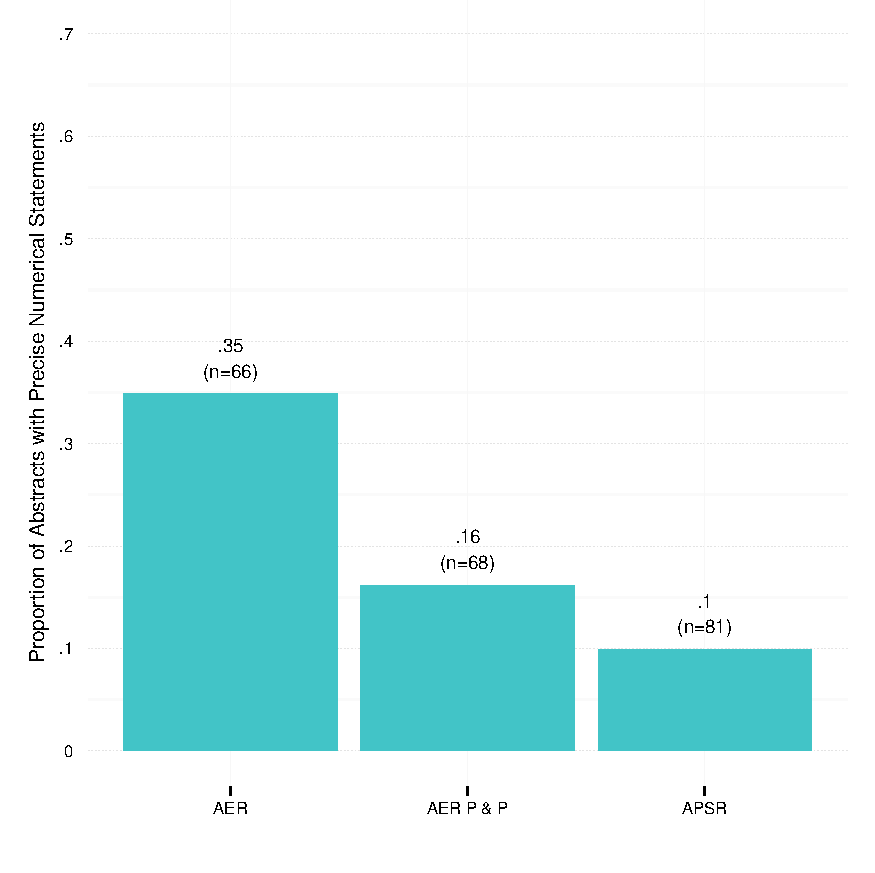
\includegraphics[scale=.75]{../figs/apsr_aer.pdf}
\label{fig:summary}
\end{figure}

Only about 10\% of the empirical articles in recent volumes of \emph{APSR} have abstracts with precise quantitative statements, similar to the percentage for \emph{AER} \emph{P \& P}. The comparable number for \emph{AER} is 35\% (see Figure~\ref{fig:summary}). None of the numbers are appealing, but the numbers for \emph{APSR} stand out. The frequency of coarse summaries of empirical results in abstracts is, however, an imperfect indicator of the dominance of NHST inspired reasoning. The disparity between \emph{APSR} and \emph{AER} likely also stems from a lack of widely understood measures in political science. For instance, in Economics, variables like unemployment, inflation, GDP, etc. are widely understood and studied. In political science, only turnout comes close to being widely understood. In all, the data shed much needed, but still weak, light on the issue. However, it is our hope that this note will stimulate discussion about social scientific writing, and increase efforts to address (what we contend is) the root cause of a particularly common coarse description—categorical statements around statistical significance.

\clearpage
\bibliographystyle{apsr}
\bibliography{quantbib}

\end{document}
